\usepackage{graphicx}


\chapter{Onderzoeks plan}\label{ch:onderzoekPlan}


\section{Inleiding en aanleiding}\label{sec:inleiding-en-aanleiding}% TODO: Wellicht weglaten en inleiding kaal laten beginnen
In het vorige hoofdstuk~\ref{ch:opdracht} is de opdracht voor dit onderzoek duidelijk uitgeschreven. In dit hoofdstuk wordt uitgewijd over hoe deze opdracht wordt onderzocht met als resultaat een methode die geimplementeerd kan worden.

[NOTE:]Gezien de te ontwikkelen module een zekere impact zal hebben op de manier van werken binnen EagleScience is het goed om een solide plan van aanpak te hebben voor er daadwerkelijk begonnen wordt aan het ontwikkelen en uitrollen van de module. Hieronder worden de vershillende fasen van het project beschreven met daarbij de geschatte tijd die het gaat duren. Het project vangt aan in september 2021 aan en de oplevering van de module is gepland voor wordt gezet op eind januari 2022. Om hieraan te kunnen voldoen moeten er een aantal milestones worden gedefinieerd. Hieronder volgt een globale beschrijving van de milestones, opleveringen, en methodes die gebruikt worden om de milestone te halen.


\section{Probleemanalyse}\label{sec:probleemanalyse}
Eaglescience heeft de ambitie om te groeien en om deze reden is er de behoefte om een aantal taken te automatiseren en inzichtelijker te maken. Een belangrijk speerpunt binnen de organisatie is het leveren van veilige software. Eén van de taken die geautomatiseerd moeten worden is het inventariseren van het gebruik van externe bibliotheken en de staat van deze bibliotheken. Op dit moment wordt de analyse namelijk door de ontwikkelaars zelf gedaan, naast dat dit realtief veel tijd kost is er geen centraal overzicht in de bevindingen die middels de analyse gevonden zijn. Om toch een duidelijk beeld te vormen voor zowel de ontwikkelaars als de projectmanagers dient er een module ontwikkeld te worden die middels een periodieke actie een analyse uitvoerd worden op projecten die in het beheer zijn van EagleScience. De resultaten van deze geautomatiseerde analyse moet zichtbaar worden in de op dit moment in ontwikkeling zijnde portal. Door deze resultaten inzichtelijk te hebben is er een beter beeld in mogelijk kwetsbaarheden die meekomen in bibliotheken van derden.

Het onderzoek moet een methode opleveren die implementeerbaar is in de huidige manier van werken binnen Eaglescience. Het moet gebruik maken van de huidige buildstraat om informatie te verkrijgen en de verkregen informatie moet op een ordelijke manier worden getoond in de portal. Daarnaast moeten er notificaties worden gegeven middels mail of rocketChat aan de betrokkenen per project. Uit dit resultaat wordt de volgende onderzoeksvraag opgebouwd:

"Welke methode is te implementeren voor het verkrijgen van informatie van externe bibliotheken op het gebied van kwetsbaarheden, zonder dat de dagelijkse manier van werken en de huidige dev-stack wordt beinvloed?"

Eaglescience heeft als doel het ontwikkelen van goede en veilige software op een dus danige manier dat het voor de klant betaalbaar blijft. Om deze doelstellingen te halen streeft het complete team in het zo effieciënt mogelijk werken om de wensen van een klant om te zetten in werkende applicatie. Er moet dus altijd een overweging gemaakt worden welke taken er uitgevoerd kunnen worden binnen het budget. Vaak zijn ontwikkeltaken declarabel en dus kosten dekkend. Er zijn ook taken die niet direct zichtbaar resultaat geven, maar wel gewenst zijn om te doen. Deze taken zijn vaak moeilijk te verkopen aan een klant of zijn zelfs niet declarabel. Het is dus zaak om deze taken nog sneller en efficienter uit te voeren dan al het geval is. Daarom is er dan ook de wens om een aantal van deze taken te automatiseren. Dit onderzoek gaat over het automatiseren van één van die taken welke periodiek terugkomt, waarbij een ontwikkelaar een analyse uitvoerd op externe bibliotheken om op deze manier potentiele kwetsbaarheden te verwijderen en hier vervolgens een rapport op uitbrengt. Dit is nodig om een grotere zekerheid te bieden dat de applicaties die we uitrollen veilig zijn.

Bij projecten waar actief op ontwikkeld wordt er gemiddeld iedere 2 maand een analyse uitgevoerd waarbij een ontwikkelaar ongeveer 8 uur bezig is. EagleScience heeft nu $\pm$ 17 projecten in haar behaar waarvan er aan 8 actief wordt ontwikkeld. Om de analyse te doen voor alle actieve projecten is er 128 uur per jaar nodig om dit uit te voeren op de frequentie zoals die nu is. EagleScience maakt naast een groei ook een verandering door, doordat het procedures vast legt waarbij er processen binnen projecten worden opgesteld en gewaarborgt. Een van de veranderingen is dat er vaker, aan het einde van een spring tijdens een uitrol, een analyse op kwetsbaarheden in externe bibliotheken moet worden uitgevoerd. deze verhoging in frequentie heeft tot gevolg dat in plaats van 6 aantal analyses*8aantal uren *8aantal projecten  = 384 uur,  24 * 8*8 = 1664 uur in beslag zal nemen.

Het gestelde probleem is dan ook de ontwikkeling en implementatie van een methode die automatisch en periodiek een analyse uitvoerd op de door eaglescience beheerde projecten. De analsye moet kwetsbaarheden op een overzichtelijke manier weergeven in de portal van EagleScience. Daarnaast moet er een notificatie worden verstuurd naar betrokkenen met daarin een samenvating en/of een dreigende situatie.
Door het implementeren van deze module zou het betekenen dat een ontwikkelaar praktisch geen tijd bezig is aan de analyse zelf, maar de tijd die vrijgekomen is te spenderen aan het updaten en daarmee veiliger maken van de software.


\section{Probleemstelling}\label{sec:probleemstelling}
Hoewel veilige software ontwikkelen niet alleen hangt aan een analyse van externe bibliotheken draagt dit wel bij aan het gehele plaatje. Daarnaast is de groei van EagleScience een andere reden om deze module te implementeren. Zeker als er meegenomen wordt dat het aantal manuren gelijk kan blijven ondanks dat er een vermeerdering van de aantal analyses die uitgevoerd gaan worden. Om dit te bewerkstelligen moet er onderzoek gedaan worden naar een methode waarbij er periodiek een analyse moet worden gedaan op externe bibliotheken. Waarbij er bij iedere uitrol een verversing van de inputdata moet zijn en er op een geselecteerd moment een analyse moet worden gedaan op deze vernieuwde informatie.


\section{Doelstellingen}\label{sec:doelstellingen}
De doelstellingen voor dit onderzoek is dan ook om een methode te vinden die voldoet aan het oplossen van bovenstaand probleem zonder dat deze in de weg zit van de huidige manier van werken. Ook moet de methode passen bij de huidige dev-stack die binnen EagleScience wordt gehanteerd.

[NOTE: Verder uitbreiden en anders samenvoegen met Probleemstelling]


\section{Centrale vraagstelling}\label{sec:centrale-vraagstelling}

De centrale vraag in het onderzoek moet zijn: "Welke methode is het meest geschikt voor het geautomatiseerd en periodiek uitvoeren van een SOUP analyse?
Verder uitbreiden.


\section{Stakeholdersanalyse}\label{sec:stakeholdersanalyse}
Binnen EagleScience zijn er een aatal stakeholders die belang hebben bij deze nieuwe methode en module. Naast de stakeholders binnen Eaglescience is er nog een stakeholder in de vorm van de klant. Hoewel de klant niet actief is in de ontwikkeling van deze methode/module. Zij hebben er wel degelijk belang bij het resultaat en dienen ook genoemd te worden.

\subsection{Dagelijks bestuur (intern)}\label{subsec:dagelijks-bestuur-(intern)1}
Het dagelijks bestuur ziet vooral voordelen in het inzicht krijgen van kwetsbaarheden op een overzichtelijke manier, zodat ze kunnen sturen in het gebruik van biblioteken of andere technologiën. Ook al zullen er kosten die niet direct terug te verdienen zijn gemoeit met de ontwikkeling van een nieuwe methode.
Echter, zien zij ook kosten gemoeid met de verandering.
Door de manier van werken dienen deze kosten terug verdient te worden door werkzaamheden binnen andere projecten.
De CTO ziet vooral tijdswinst zodat de time-to-market voor andere projecten hoger ligt en dus meer verdient kan worden.

\subsection{Projectmanagers (intern)}\label{subsec:projectmanagers-(intern)1}
Project managers krijgen op dit moment een update over de staat van kwetsbaarheden tijdens stand-ups en aan het einde van een sprint tijdens de sprint demo's.
De nieuwe module biedt ze de mogelijkheid om up-to-date informatie on-demand te verkrijgen.
Op de vraag of het het waard is dat een aantal ontwikkelaars tijd kwijt zijn in testen en meedenken over de module weegt volgens hen op tegen de voordelen die de module in de toekomst kan brengen.

\subsection{Ontwikkelteam (intern)}\label{subsec:ontwikkelteam-(intern)1}
Het ontwikkelteam wil graag meedenken en meewerken aan een oplossing, gezien zij de gene waren die handmatig de analyse uitvoerden.
Zij zien voor een oplossing voor een taak dat veel tijd in beslag nam en afleide van de daadwerkelijke taak.

\subsection{Klant (extern)}\label{subsec:klant-(extern)1}
Als laatste de klant welke een passieve stakeholder is gezien zij niet direct betrokken zijn bij de ontwikkeling van de module maar wel verbeteringen genieten in de zin van veilige en betrouwbare software.

\subsection{Stakeholder analyse}\label{subsec:stakeholder-analyse1}
\begin{figure}[H]
    \myfloatalign
    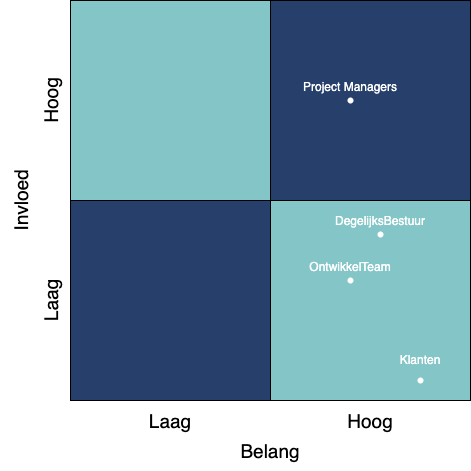
\includegraphics[width=10cm]{gfx/stakeholderanalyse}
    \caption{StakeHolders Analyse}
    \label{fig:StakeholderAnalyse1}
\end{figure}
[NOTE]Figuur stakeholder analyse nog aanpassen.
Zoals te zien is in figuur~\ref{fig:StakeholderAnalyse1} zijn de projectmanager, het ontwikkelteam en de klanten het meest gebaad bij een nieuwe module voor de analyse van kwetsbaarheden.
Echter zijn de klanten niet tot bijna niet betrokken bij de ontwikkeling van de module maar hebben er indirect wel belang bij omdat de software die voor hen ontwikkeld wordt veiliger wordt door het voeren van een geautomatiseerde analyse.
Door deze analyse worden alleen de requirements meegnomen die intern zijn opgenomen.
•


\section{Theoretisch kader}\label{sec:theoretisch-kader}
Het theoretisch kader waarmee in dit onderzoek wordt gewerkt bestaat uit een aandal hoofdelen. Het eerste hoofdeel is de huidige situatie binnen EagleScience hierbij wordt inbegrepen de dagelijkse werkwijze, de gebrukte dev-stack en de manier waarop er op dit moment wordt uitgerold. Het tweede hoofddeel is zijn artikelen(uitzoeken welke ) waarin bestpractices, adviezen vanuit ervaringsdeskundigen en erkende methoden om SOUP analyses te doen beschreven staan. Het laatste hoofddeel is de theorie waarin beschreven wordt waarom het wenselijk is om uberhaubt analyses te doen. In de laatste sectie van dit hoofdstuk staat een literatuurlijst met de beoogde gebruikte literatuur.


\section{Conceptueel model}\label{sec:conceptueel-model}
In figuur () is het conceptueel model opgenomen dat behoordt bij dit onderzoek. Dit model beoogt om de validaliteit van het onderzoek transparant te maken, en geeft de samenhang tussen de verschillende begrippen weer.

Het kernbegrip van het conceptueelmodel is "de implementatie van een methode voor het geautomatiseerd uitvoeren van een SOUP analyse op de gebruikte bibluitheken door EagleScience" Binnen het kernbegrip zijn sub begrippen te ontleden die van belang zijn binnen het onderzoek. Allereest dient het begrip "gebruikte bibliotheken door EagleScience worden bekeken, dit om een kader te verschaffen in welke talen en tools gebruikt worden. Het begrip SOUP analyse is een onderdeel van het onderzoek om theoretische kennis te verkrijgen over het begrip en daarmee input te geven over het laatste begrip "de implementatie van een methode voor een geautomatiseerde SOUP analyse. De twee eerst genoemde begrippen geven een input voor het laatste begrip.


\section{Deelvragen}\label{sec:deelvragen}
Aan de hand van het conceptueel model en de hoofdvraag zijn er de volgende deelvragen voor dit onderzoek opgesteld:
\textbf{Dev-stack binnen Eaglescience}
\begin{itemize}
    \item Welk proces wordt er binnen Eaglescience gebruikt om software te ontwikkelen en hoe resulteert dit is een dagelijkse werkwijze?
    \item Wat zijn de meest gebruikte ontwikkeltalen en frameworks die binnen EagleScience worden toegepast?
    \item Welke tooling wordt er gebruikt binnen EagleScience? [NOTE relevant?]
    \item Hoe wordt er binnen EagleScience software uitgerold?
\end{itemize}

\textbf{Theorie over SOUP}
\begin{itemize}
    \item Wat is veilige software?
    \item Wat is SOUP?
    \item Wat dragen externe bibliotheken en dus ook potentieel SOUP bij aan de ontwikkeling van software?
    \item Wat zijn de gevaren van het gebruik van SOUP?
    \item Wordt er ergens bijgehouden of een dependency/component) een kwetsbaaheid bevat?
    \item Wat relateert SOUP tot software veiligheid binnen EagleScience?
\end{itemize}


\textbf{Methodes om een SOUP analyse te doen binnen de Dev-stack van EagleScience}
\begin{itemize}
    \item Welke tools bestaan er om dependency informatie uit een sbt en npm project te halen?
    \item Hoe zijn de tools in te zetten in de huidige projecten?
    \item Welke output wordt er verkregen van de tools?
    \item Welke manieren zijn er om uit de huidige pipeline informatie over de deploy te halen?
    \item Wat zijn hier de voor en nadelen van?
\end{itemize}


\section{Onderzoeksontwerp}\label{sec:onderzoeksontwerp}
Gezien de grote hoeveelheid deelvragen die benoemd zijn op basis van de onderzoeksvraag en het conceptueel model is het verstandig om het onderzoek in kleinere onderzoeken te verdelen. Door het op te delen in deelonderzoeken kan het kader beter worden vastgesteld en zal er minder snel "teveel" worden onderzocht. De deel onderzoeken zal op de volgende manier worden opgesplitst:
\begin{enumerate}
    \item \textbf{Werkwijze en dev-stack Eaglescience} Dit onderzoek moet inzicht geven in de dagelijkse manier van werken binnen EagleScience en de daarbij gebruikte dev-stack. Het resultaat is inzicht in hoe EagleScience applicaties ontwikkeld en hoe deze uitgerold wordt. Daarnaast is er inzicht in hoe er op dit moment een SOUP analyse wordt gedaan.
    \item \textbf{Theorie SOUP analyses} Om een methode te kunnen ontwikkelen is er een theoretische basis nodig. Dit onderzoek geeft inzicht in de theoretische basis en het belang om een analyse te doen. Daarnaast wordt er uitgezocht hoe er het beste een analyse gedaan kan worden.
    \item \textbf{Methode voor Soup analyse binnen EagleSciende} Door inzichten uit voorgaande onderzoeken te combineren en nieuwe kennis toe te voegen is er een ontwerp voor een implementatie die aan de opdracht voldoet.
\end{enumerate}

\subsection{strategie}\label{subsec:opstrategie}
Om de drie onderzoeken die hierboven beschreven zijn goed uit te kunnen voeren zijn er de volgende strategien bedacht die ervoor zorgen dat er een betrouwbaar resultaat is waar verder mee gewerkt kan worden.
Voor het onderzoek binnen de huidige situatie binnen EagleScience wordt interne documentatie geraadpleegd aangevuld met vraag gesprekken met collega's die met het onderwerp te maken hebben. Deze gespreken zullen worden gehouden in delen gezien de manier waarop er binnen EagleScience gewerkt wordt. (heeft te maken met het aantal niet declarabele uren die ieder persoon wel of niet heeft). Het onderzoek naar de theorie van SOUP analyses wordt uitgevoerd middels een deskresearch waarbij in literatuur gezocht wordt naar methoden om de analyse te doen. Daarnaast wordt er een selectie gemaakt in tools die al ontwikkeld zijn die bruikbaar zijn voor het einddoel van de opdracht. In het laatste onderzoek wordt gekeken naar een method die past bij de huidige manier van werken binnen eaglescience, en de tools die gevonden zijn. Ook wordt er een ontwerp gemaakt hoe de methode eruit komt te zien er welke data dit oplevert waarna er een module ontwikkeld kan worden die deze data inzichtelijk maakt voor de stakeholders.


\section{bronnen}\label{subsec:bronnen}
De bronnen die gebruikt zijn voor de onderzoeken zijn in de komende subsecties per onderzoek genoemd

\subsection{Onderzoek EagleScience}
\begin{itemize}
    \item \textbf{151030 F04B Proces Flow Chart ES\_V1.0\_TN.pdf} een document dat de workflow beschrijft die binnen EagleScience gehanteerd wordt.
    \item \textbf{200121\_Policy Manual\_ES\_V6 signed.pdf} ISO handboek waarin de bedrijfsvoering binnen EagleScience wordt beschreven.
    \item \textbf{https://www.scala-lang.org} Website met informatie over de taal gebruikt door EagleScience
    \item \textbf{https://angular.io} Website van Angular gebruikt door EagleScience om frontends te ontwikkelen
    \item \textbf{https://about.gitlab.com} Gitlab website
    \item \textbf{https://www.atlassian.com/software/jira} Jira Website
    \item \textbf{https://www.atlassian.com/software/confluence} Confluence website
    \item \texbf{https://Jenkins.io} Website van Jenkisn welke door EagleScience wordt gebruikt als build tool.
    \item \textbf{Collega's} Interviews met collega's over het gebruik van de verschillende tooling binnen EagleScience
\end{itemize}

\subsection{Onderzoek SOUP theorie}

\subsection{Onderzoek implementatie SOUP analyse}


\section{planning}\label{subsec:planning}

\subsection{Requirements analyse \textbf{september 2021}}\label{sec:requirements-analyse}
Na het ontvangen van de opdracht dient er onderzocht te worden of er naast de eisen die door de CTO in de opdracht zijn gezet nog andere eisen zijn binnen EagleScience. Hiervoor zal er onderzocht worden welke betrokkenen er zijn en welke belangen en wensen zij hebben. Na het houden van interviews zullen alle wensen tegen elkaar worden afgewogen. Dit zal leiden tot een document waarin alle belangrijke requirements worden geprioriteerd volgens de MoSCoW-methode.

\textbf{Methode:} Intake gesprek met opdrachtgever, interviews met betrokkenen, enquete voor ontwikkelaars.

\textbf{Resultaat:} Applicatie requirements document.

\subsection{Vooronderzoek \textbf{september 2021 - oktober 2021 }}\label{sec:onderzoek}
Om de requirements om te kunnen zetten naar een ontwerp zal er onderzoek gedaan worden naar de huidige manier van ontwikkelen en compileren van de software. Een onderzoek naar begrippen binnen het domein SOUP is een voorwaarde om vervolgens onderzoek te kunnen doen naar methodes om analyses te kunnen doen op software die EagleScience maakt ten opzichte van SOUP. De resultaten van het vooronderzoek zullen worden gebruikt als input.
Om meer kennis en verdieping te krijgen in de materie rondom de nieuwe module zullen er een aantal onderzoeken worden uitgevoerd.


Er is onderzoek nodig naar de volgende onderwerpen:
\begin{itemize}
    \item \textbf{Architectuur binnen EagleScience} Werkwijze en ontwikkel stack van EagleScience met daarin specifiek onderzocht hoe er omgegaan wordt met het voorkomen van onveiligheden in de geleverde software
    \item \textbf{Externe bibliotheken gebruik en het gevaar} Onderzoek naar waarom er externe bibliotheken worden gebruikt en het gevaar hiervan.
    \item \textbf{Soup Analyse} Door te kijken naar de kwetsbaarheden in de externe bibliotheken kan er beter worden nagegaan of er kwetsbaarheden in de software zitten. Dit onderzoek zal in gaan op het bestaan van methodes om SOUP analyses te doen. En een mogelijkheid om dit (deels) geautomatiseerde te doen.
\end{itemize}

\textbf{Methode:} Bureau onderzoek, interviews met specialisten, meedoen aan en/of terugkijken van conferenties

\textbf{Resultaat:} Inzicht in het begrip SOUP en software veiligheid als ook een idee voor een mogelijke implementatie van de oplossing die voor EagleScience de beste is zonder veel impact op de huidige manier van werken te hebben.

\subsection{Initieel ontwerp \textbf{oktober 2021 - november 2021 }}\label{sec:initieel-ontwerp}
Er zal een ontwerp worden gemaakt waarin vast gelegd is welke requirements er beslist in de module moeten zitten en de uitwerking van deze. Evenals een ontwerp van de architectuur en het datamodel. Naast de module zal er ook een ontwerp gemaakt worden voor een ontwikkel/test omgeving om de module continue te kunnen testen zonder dat dit de huidige buildstraat beinvloed. Dit laatste is van belang om zo min mogelijk storingen te veroorzaken in de dagelijkse gang van zaken bij al lopende projecten. Het eerste ontwerp zal als leidraad dienen voor de implementatie waarin afgeweken kan worden als dit nodig blijkt tijdens de implementatie sprints.

\textbf{Methode:} Overleggen met ontwikkelaars, huidige omgeving onderzoeken op mogelijkheden en architectuur.
\textit{wellicht nog toevoegen als resultaten: blokdiagram van oplossing/architectuur; sequence diagram om te komen van analyse tot rapportage (er is een handig tooltje om deze diagrammen te tekenen: https://bramp.github.io/js-sequence-diagrams/)}
\textbf{Resultaat:} Eerste ontwerp in de vorm van een datamodel, blokdiagram van architectuur voor de oplossing, als ook een sequence diagram om van analyse tot rapportage te komen.

\textit{4.4: Gebruik hier of de template ontwikkel omgeving voor (aparte branch/taak); of de portal ontwikkelomgeving
4.4: Voeg rij resultaat toe: klaar voor review of gereviewde}

\subsection{Implementatie en Testen \textbf{november 2021 - januari 2022 }}\label{sec:implementatie-en-testen}
Om te kunnen beginnen aan de implementatie is er een ontwikkel/ test omgeving nodig die het mogelijk maakt om zonder invloed op de dagelijkse werkzaamheden van EagleScience een module te kunnen ontwikkelen. Deze zal eerst worden opgezet. Als test projecten zullen snapshots worden gebruikt van de daadwerkelijke projecten dit om een zo accuraat mogelijke test omgeving te hebben. Zoals in de opdracht beschreven dient de nieuwe module een onderdeel te zijn van de bestaande portal. Er zal dan ook direct samen worden gewerkt met het team die daar op het moment mee aan het ontwikkelen is. Tijdens de implementatie zal er ook worden gedocumenteerd wordt hoe de module werkt en welke procedures hier in worden gevolgd. Dit document biedt ontwikkelaars de mogelijkheid om dit door te nemen als on-boarding en referentie.

\textbf{Methode:} Agile scrum sprints met iedere 2 weken een oplevermoment en demo als ook een reflectie op de sprint.
\textbf{Resultaat:} Werkende en geteste applicatie die klaar is om uitgerold te worden.

\subsection{Uitrollen en documentatie \textbf{januari 2022 - februari 2022 }}\label{sec:uitrollen-en-documentatie}
Nadat de implementatie van de meest kritische requirements is afgerond zal er worden begonnen met het uitrollen van de module en het testen door een geselecteerde groep gebruikers. De feedback wordt bekeken en meegenomen in de evaluatie. Mocht het nodig zijn dan zal er accuut actie worden ondernomen om deze wijzigingen aan te passen. Mochten er wensen zijn die kunnen wachten dan zal er worden overwogen om deze mee te nemen in de volgende iteratie van het project. (de verwachting is dat de module die hier beschreven wordt verder zal worden uitgebreid met de diverse mogelijkheden om betere en veiligere software te ontwikkelen.) Daarnaast zal ook de documentatie verder worden afgerond.
\textbf{Methode:} Interviews met stakeholders met een analyse over de nieuwe requirements.

\textbf{Resultaat:} Uitegrolde en gedocumenteerde applicatie


\section{Literatuurlijst (APA)}

zie : https://www.topscriptie.nl/plan-aanpak-stappenplan-en-structuur/
In het vorige hoogdstuk is de opdracht die is meegegeven vanuit de CTO uitvoerig te lezen. in de






